\section{Graph Transformations}\label{sec:gratra}

Graph transformation is a systematic, rule-based transformation technique. It has a solid research foundation \cite{Handbook-GG-I} and applications in many areas of computer science.\\
A graph is a type $(N,E)$ where $N$ is a set of nodes and $E \subseteq N \times Lab \times N$ a set of labelled edges.  
%Nodes are not labelled by definition, but can have outgoing edges pointing to itself. These edges are called \emph{self-edges} of a node.
Nodes are graphically represented as black bordered boxes and edges as black arrows.
%Self-edges can be represented as labels of nodes (depicted inside the box), or as arrows with the same start and end node. An example of this is shown in Figure \ref{fig:edge_types}.a.\\
A graph production system (GPS) is a set of \emph{graph production rules}, each of which can transform a \emph{source graph} into a new graph called the \emph{target graph}. The rule specifies both the conditions under which it applies and the changes it makes to the source graph. Technically, a graph production rule consists of two partially overlapping graphs, a \emph{left hand side} and a \emph{right hand side}, and a set of \emph{negative application conditions}, which are also (connected) graphs partially overlapping with the left hand side.

Graph transformations provide an attractive visual representation. In our visual representation of a rule used in this paper (which is taken from the {\sc GROOVE} tool \cite{Rens03d}) we combine all elements together in one graph, made up of four types of elements:

\begin{figure}
	\begin{center}
		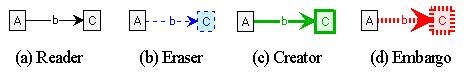
\includegraphics[scale=0.5]{edge_types.jpg}
	\end{center}
	\caption{The graph production rule elements}
	\label{fig:edge_types}
\end{figure}

\begin{list}{$\bullet$}{}
\item \emph{Readers}: elements that are used for matching; are depicted as with black borders and arrows (see Figure \ref{fig:edge_types}.a);
\item \emph{Erasers}: elements that will be erased during the transformation are depicted with thin dashed borders and arrows (see Figure \ref{fig:edge_types}.b);
\item \emph{Creators}: elements that will be created during transformation are depicted with thick light gray borders and arrows (see Figure \ref{fig:edge_types}.c);
\item \emph{Embargoes}: elements that are not allowed to be present in the graph when the rule is matched are depicted with dashed, dark gray edges (see Figure \ref{fig:edge_types}.d)
%\footnote{For the more knowledgeable in the field of graph transformations: readers and erasers represent the left-hand-side (LHS); readers and creators represent the right-hand-side}. NACS are elements that may not have a matching in the source graph.
\end{list}

Given an operational semantics specified in graph transformation rules, the system can be (manually or automatically) simulated, which results in a labelled transition system (LTS), where the states are graphs, and the transitions are rule applications. In the context of this paper, the graphs contain the static structure of an AFJ program and a part that represents run-time information. The graph production system is an operational semantics of the FAJ language. This means that, by simulation, we can generate an LTS of the execution of an FAJ program. 

%For the purpose of the rules used in this paper, it actually does not make an essential difference what precise graph transformation formalism is used, since the rules can be formulated in either algebraic or algorithmic formalisms \cite{Handbook-GG-I}. In fact, we have used GROOVE \cite{Rens03d} as a tool to carry out the transformations and generate the state spaces; this means that the actual rules have been defined in the Single-Pushout approach \cite{Ehri+97}. Since the point of this paper is to illustrate an application of graph transformations, we omit the details of the formalism.\\
